\begin{document}

\def\lecturename{嵌入式技术}

\title{\insertlecture}

\author{邢超}

\institute
{
  西北工业大学航天学院
}

%\mode<presentation>{\subject{嵌入式系统}}

%  start a lecture  --------------------------
\lecture[EC]{嵌入式技术}{}
\subtitle{GNU/Linux 进程}
\date{2015}


%\setbeamertemplate{background}{\pgfimage[width=\paperwidth,height=\paperheight]{image/flower}}
%\setbeamercovered{transparent}
%\mode<presentation>{\beamerdefaultoverlayspecification{<+->}}

\begin{frame}
  \maketitle
\end{frame}

%\begin{frame}{课程内容}
%\begin{center}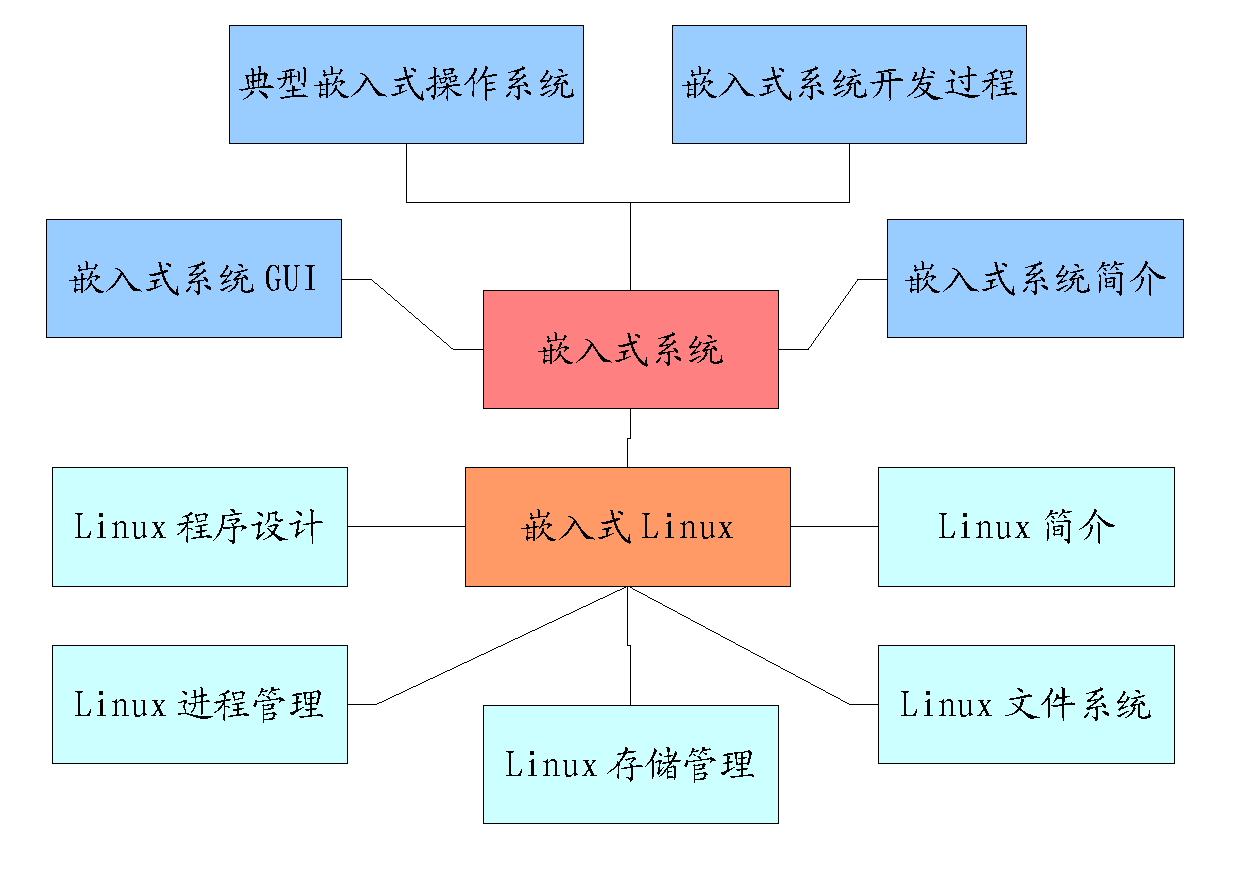
\includegraphics[height=0.8\textheight]{image/content.pdf}\end{center}
%\end{frame}

\section{Linux内核特点}

\begin{frame}{宏内核结构与微内核结构}
\begin{center}\pgfimage[width=0.9\columnwidth]{image/linuxkernel}\end{center}
\end{frame}

%\begin{frame}{特点}
%\begin{itemize}
%\item 进程管理
%\item 中断管理
%\item 系统调用
%\item 进程间互斥
%\item 进程间通信
%\end{itemize}
%\end{frame}

\begin{frame}{系统调用}
\begin{center}\pgfimage[width=0.9\columnwidth]{image/linuxsystemcall}\end{center}
\end{frame}

\begin{frame}{中断处理与定时器}
     \begin{itemize}
     \item 中断
           \begin{itemize}
           \item 外部设备生成的中断
           \item 软件程序生成的中断(陷阱 trap)
           \end{itemize}
     \item 中断描述符表(IDT)
           \begin{itemize}
           \item 中断编号
           \item 入口指针
           \end{itemize}
     \end{itemize}
\end{frame}


\section{进程调度}
\begin{frame}{进程}
\begin{itemize}
\item 进程是执行程序的一个实例
\item 进程和程序的区别	
\begin{itemize}
\item 几个进程可以并发的执行一个程序,这些进程共享内存中程序正文的单一副本,但每个进程有自己的单独的数据和堆栈区
\item 一个进程可以顺序的执行几个程序,一个进程可以在任何时刻执行新的程序,并且在它的生命周期中可以运行几个程序
\end{itemize}
\end{itemize}
\end{frame}

\begin{frame}{进程状态}
\begin{itemize}
\item 就绪态:
\begin{itemize}
\item 进程已经获得所有所需的其他资源;
\item 正在申请处理机资源,准备运行。
\end{itemize}
\item 阻塞态(休眠状态,或等待状态):
\begin{itemize}
\item 进程因需要等待所需资源而放弃处理机;
\item 或者进程本不拥有处理机,且其他资源也没有满足(从而即使得到处理机资源也不能开始运行)。
\end{itemize}
\item 运行态:
\begin{itemize}
\item 指进程得到了处理机,不需要等待其他任何资源,正在执行的状态;
\item 此时进程才可使用申请的资源
\end{itemize}
\end{itemize}
\end{frame}

\begin{frame}{进程调度}
\begin{center}\pgfimage[width=0.9\columnwidth]{image/linuxstate}\end{center}
\end{frame}


\begin{frame}{进程编号}
\begin{itemize}
\item 进程以进程号PID(process ID)作为标识。任何对进程的操作都要有相应的PID号。
\item 每个进程都属于一个用户,进程要配备其所属的用户编号UID。
\item 每个进程都属于多个用户组,所以进程还要配备其归属的用户组编号GID的数组 。
\end{itemize}
\end{frame}

% \begin{frame}{进程上下文}
% \begin{itemize}
% \item 进程控制块:PCB包括进程的编号、状态、优先级以及正文段和数据段中数据分布的大概情况。
% \item 正文段(text segment):存放该进程的可执行代码。
% \item 数据段(data segment):存放进程静态产生的数据结构
% \item 用户堆栈(stack)
% \end{itemize}
% \end{frame}

\begin{frame}{进程切换:进程上下文}
\begin{itemize}
\item 运行进程的环境称为进程上下文(context),包含了进程执行需要的所有信息
\item 包括:
\begin{itemize}
\item 用户地址空间:包括程序代码,数据,用户堆栈等
\item 控制信息:进程描述符,内核堆栈等
\item 硬件上下文
\begin{itemize}
\item 通用寄存器,如eax,ebx等
\item 系统寄存器,如eip,esp,cr3等等
\end{itemize}
\end{itemize}
\end{itemize}
\end{frame}

\begin{frame}{进程表 (process table) }
\begin{center}\pgfimage[width=0.9\columnwidth]{image/linuxprocessPCB}\end{center}
\end{frame}

\begin{frame}{进程的创建}
\begin{itemize}
\item 系统启动时,自行创建了0号进程(init\_task())。作为一切其他进程的父进程。
\begin{itemize}
\item 系统调用fork
\item 系统调用vfork
\item 系统调用clone
\end{itemize}
\item 执行一个新程序
\begin{itemize}
\item 系统调用exec
\end{itemize}
\item 终止进程
\begin{itemize}
\item 系统调用exit
\item 进程也可以因收到信号而终止
\end{itemize}
\end{itemize}
\end{frame}



\def\lstlistingname{例}
\begin{frame}[containsverbatim]{fork.c}
\begin{lstlisting}
#include <stdio.h>
#include <stdlib.h>
#include <sys/types.h>
#include <unistd.h>
int main(int argc, char* argv){
  printf("father start\n");
  pid_t self=getpid();
  pid_t pid=fork();//child process start here
  printf("child start\n");
  if(pid>0){
    printf("Father: %d,child:%d\n",self,pid);
    exit(0);
  }
  if(pid==0){
    printf("Child: %d,father: %d\n",(int)getpid(),self);
    exit(0);
  }
  if(pid<0){
    printf("Error,Create Failure!\n");
    exit(1);
  }
}
\end{lstlisting}
\end{frame}


\begin{frame}{fork}
\begin{itemize}
\item 调用fork的进程称为父进程
\item 新进程是子进程
\item 子进程的地址空间是父进程的复制,一开始也是运行同一程序。
\item 为父子进程返回不同的值
\end{itemize}
\end{frame}

\begin{frame}{写时复制技术}
\begin{itemize}
\item 背景
\begin{itemize}
\item 很多情况下,子进程从fork返回后很多会调用exec来开始执行新的程序
\item 这种情况下,子进程根本不需要读或者修改父进程拥有的所有资源。
\item 所以fork中地址空间的复制依赖于Copy On Write技术,降低fork的开销
\end{itemize}
\item 实现方法
\begin{itemize}
\item 写时复制技术允许父子进程能读相同的物理页。
\item 只要两者有一个进程试图写一个物理页,内核就把这个页的内容拷贝到一个新的物理页,并把这个新的物理页分配给正在写的进程
\end{itemize}
\end{itemize}
\end{frame}

\begin{frame}{进程间关系}
\begin{center}\pgfimage[width=0.9\columnwidth]{image/linuxprocess_parent_children}\end{center}
\end{frame}

\section{信号}
\begin{frame}{Linux系统信号}
\begin{itemize}
\item 信号主要用于通知进程异步事件的发生。 
\item 进程可以用kill或killpg系统调用向另一个进程发信号。
\item 进程可以通过提供信号处理函数来取代对于任意信号的缺省反应,这种缺省反应一般都是终止进程。
\item 信号发生时,内核中断当前的进程,进程执行处理函数来响应信号,结束后恢复正常的进程处理。
\end{itemize}
\end{frame}

\section{进程间通信}
\begin{frame}{进程间通信}
     \begin{itemize}
     \item 管道机制:
           \begin{itemize}
           \item 源进程向管道写数据,而内核会自动将这些数据引导向目标进程
           \item 写之前必须关闭读管道,反之亦然。
           \end{itemize}
     \item 先入先出机制:
            \begin{itemize}
            \item FIFO为“first in,first out”的简写,指一个在磁盘上的文件,它可以被所有进程所共享。
            \item FIFO与一般文件不同,它还使用了内核中的缓冲区,所以在效率上要比一般共享文件快得多。
            \item FIFO和管道都可以使用read()和write()调用来进行读写操作。
            \end{itemize}
     \item IPC(Interprocess Communication)机制:
           \begin{itemize}
           \item 信号量:用于同步
           \item 消息队列:由内核创建并维护的一个数据结构,
           \item 共亨内存:将一段内存区映射到一个进程的地址空间来实现,进程间通信不再涉及到内核
           \end{itemize}
     \end{itemize}
\end{frame}

\section{信号}
\begin{frame}{Linux系统信号}
\begin{itemize}
\item 信号主要用于通知进程异步事件的发生。 
\item 进程可以用kill或killpg系统调用向另一个进程发信号。
\item 进程可以通过提供信号处理函数来取代对于任意信号的缺省反应,这种缺省反应一般都是终止进程。
\item 信号发生时,内核中断当前的进程,进程执行处理函数来响应信号,结束后恢复正常的进程处理。
\end{itemize}
\end{frame}

\begin{frame}{Linux系统信号}
\begin{center}\pgfimage[width=0.9\columnwidth]{image/linuxsignal}\end{center}
\end{frame}

\begin{frame}{信号产生条件}
\begin{itemize}
\item 用户按下特定的键后,将向该终端前台进程组发送信号 
\item 硬件异常会产生信号:如被0除、无效内存引用等。
\item kill(2)系统调用允许进程向其他进程发送任意信号
\item kill(1)命令允许用户向进程发送任意信号。
\item 软件设置的条件,如SIGALARM。
\end{itemize}
\end{frame}

\begin{frame}{信号捕捉}
void (*signal (int signo,void (*func)(int)))(int)
\begin{itemize}
\item 其中signo是系统信号表中的信号名;
\item func的值是SIG\_IGN或SIG\_DFL或者是接到此信号后需要调用的函数地址
\begin{itemize}
\item 当func为SIG\_IGN时则向内核表示忽略此信号。
\item 当func为SIG\_DFL表示接到此信号的动作是系统默认动作。 
\item 当func为函数地址时为捕捉信号。出错则返回SIG\_ERR,成功返回信号处理配置。
\end{itemize}
\end{itemize}
\end{frame}

\begin{frame}{复杂指针详解}
\begin{center}\pgfimage[width=0.9\columnwidth]{image/signal}\end{center}
\end{frame}

\begin{frame}{发送信号}
\begin{itemize}
\item kill(pid\_t pid,int sig);
\begin{itemize}
\item pid>0是将信号发送到PID为pid的进程
\item pid=0信号发送到与发送进程在同一进程组的进程
\item pid<-1将信号发送到进程组ID等于-pid的进程
\item pid=-1Linux发到进程表中除第一个进程外的进程
\item sig=0时,不发送任何信号,但仍然执行错误检查
\end{itemize}
\item int raise(int sig);//向当前进程发送信号,
\begin{itemize}
\item 等价于kill(getpid(),sig),成功返回为0,出错为-1。
\end{itemize}
\item unsigned int alarm(unsigned int seconds);
\begin{itemize}
\item 此函数用来设置一个时间值(闹钟时间),当所设置的值被超过后,产生SIGALRM信号,默认动作是终止进程。
\end{itemize}
\item int pause(void);
\begin{itemize}
\item 可以使进程挂起,直到捕捉到一个信号。
\end{itemize}
\item unsigned int sleep(unsigned int seconds);
\begin{itemize}
\item 此函数挂起调用中的进程,直到过了预定时间或者是收到一个信号并从信号处理程序返回。 
\end{itemize}
\end{itemize}
\end{frame}


\def\lstlistingname{例}
\begin{frame}[containsverbatim]{alarm.c}
\begin{lstlisting}
#include <unistd.h>
#include <signal.h>
void handler(){
	printf("hello\n");
}
main(){
 int i;
 signal(SIGALRM,handler);
 alarm(2);
 for(i=1;i<4;i++){
   printf("sleep %d  \n",i);
   sleep(1);
 }
}
\end{lstlisting}
\end{frame}



%\lecture[]{GNU/Linux内存管理}{}
%\subtitle{内存与虚拟内存}
%\date{2007}
%\begin{frame}
%  \maketitle
%  %\titlepage
%\end{frame}

%\section{Thank you!}
%\begin{frame}
%\begin{center}
%\huge{\fontsize{60pt}{60pt}\selectfont 谢~谢~!}
%\end{center}
%\end{frame}

\section{思考}
\begin{frame}{思考}
\begin{itemize}
\item 进程与程序的区别
\item 进程间通信的实现
\end{itemize}
\end{frame}

\end{document}

